\documentclass[tikz]{standalone}

\usepackage{tikz}

\begin{document}

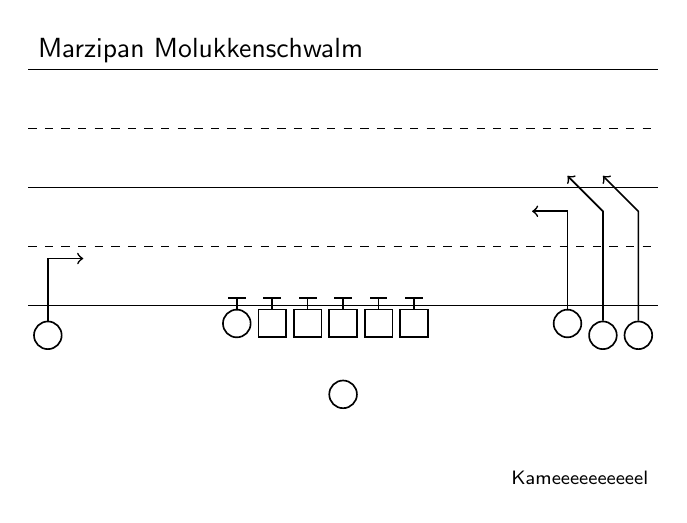
\begin{tikzpicture}[scale=0.15]
    \draw [white] (-26.66, -16) rectangle (26.66, 23.5); % bounding box

    \draw [thin]   (-26.66,  0) -- (26.66,  0); % line of scrimmage
    \draw [dashed] (-26.66,  5) -- (26.66,  5); % 5 yard gain
    \draw [thin]   (-26.66, 10) -- (26.66, 10); % 10 yard gain
    \draw [dashed] (-26.66, 15) -- (26.66, 15); % 15 yard gain
    \draw [thin]   (-26.66, 20) -- (26.66, 20); % 20 yard gain

    % name of play
    \node at (-26.66, 23.5) [anchor=north west, font=\sffamily] (name) {Marzipan Molukkenschwalm};

    % notes
    \node at (26.66, -16) [anchor=south east, font=\scriptsize\sffamily] (note) {Kameeeeeeeeeel};

    % formation
    \begin{scope}[auto, every node/.style={draw, semithick, align=center, minimum size=1em}]
        \node at (-25, -2.5) [circle]    (wr1) {};
        \node at ( -9, -1.5) [circle]    (te1) {};
        \node at ( -6, -1.5) [rectangle] (lt)  {};
        \node at ( -3, -1.5) [rectangle] (lg)  {};
        \node at (  0, -1.5) [rectangle] (c)   {};
        \node at (  3, -1.5) [rectangle] (rg)  {};
        \node at (  6, -1.5) [rectangle] (rt)  {};
        \node at ( 19, -1.5) [circle]    (wr2) {};
        \node at ( 22, -2.5) [circle]    (wr3) {};
        \node at ( 25, -2.5) [circle]    (wr4) {};

        % backfield
        \node at (  0, -7.5) [circle]    (qb)  {};
    \end{scope}

    % routes
    \begin{scope}[auto, every path/.style={semithick, ->}]
        \draw (wr1.north) -- (wr1.north |- 0, 4) -- ++( 3, 0);
        \draw (wr2.north) -- (wr2.north |- 0, 8) -- ++(-3, 0);
        \draw (wr3.north) -- (wr3.north |- 0, 8) -- ++(-3, 3);
        \draw (wr4.north) -- (wr4.north |- 0, 8) -- ++(-3, 3);
    \end{scope}

    % blocking
    \begin{scope}[auto, every path/.style={semithick, -|}]
        \draw (te1.north)      -- ++(0, 1);
        \draw ( lt.north)      -- ++(0, 1);
        \draw ( lg.north)      -- ++(0, 1);
        \draw (  c.north)      -- ++(0, 1);
        \draw ( rg.north)      -- ++(0, 1);
        \draw ( rt.north)      -- ++(0, 1);
    \end{scope}
\end{tikzpicture}

\end{document}
